\documentclass[11pt]{article} % use larger type; default would be 10pt

\usepackage{tikz}
\usetikzlibrary{calc}
\usetikzlibrary{arrows.meta}

        \newcommand\degree[0]{^{\circ}}

\title{Play with TikZ}
\author{Just Us}
%\date{} % Activate to display a given date or no date (if empty),
         % otherwise the current date is printed 

\begin{document}
\maketitle

\section{Review}
Chap 1 review hp1ans
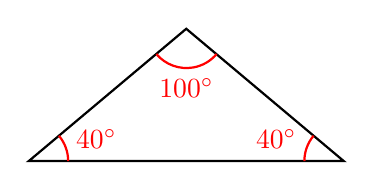
\begin{tikzpicture} 

\coordinate(A) at (0,0);
\coordinate (B) at (4,0 );
\coordinate (C) at (2,1.68);

\draw[black,thick] (A)--(B) --(C)--cycle;

\draw[red,thick] (0.5,0) arc (0:40:0.5) node[right,midway, yshift=3] {$40\degree$};
\draw[red,thick] (3.5,0) arc (180:140:0.5) node[left,midway, yshift=3] {$40\degree$};
\draw[red,thick] (1.62,1.36) arc (220:320:0.5) node[below,midway, yshift=0] {$100\degree$};

\end{tikzpicture}
\newline

Chap 1 review hp3ans
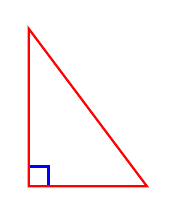
\begin{tikzpicture} 

\coordinate(A) at (0,0);
\coordinate (B) at (1.5,0 );
\coordinate (C) at (0,2);

\draw[blue,thick] (A) rectangle +(0.25,0.25);
\draw[red,thick] (A)--(B) --(C)--cycle;

\end{tikzpicture}
\newline


Chap 1 review 5

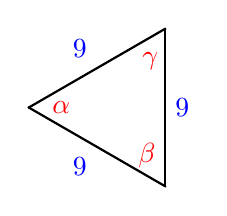
\begin{tikzpicture} 

\coordinate(A) at (0,0);
\coordinate (B) at (0,2 );
\coordinate (C) at (-1.732,1);

\draw[black,thick] (A)--(B) node[right,midway] {\color{blue}$9$};
\draw[black,thick] (A)--(C) node[below left,midway] {\color{blue}$9$};
\draw[black,thick] (C)--(B) node[above left,midway] {\color{blue}$9$};

\filldraw[black] (A) circle (.2pt) node[anchor= south east, xshift=0,yshift=3] {\color{red}$\beta$};
\filldraw[black] (B) circle (.2pt) node[anchor= north east,xshift=1,yshift=-5] {\color{red}$\gamma$};
\filldraw[black] (C) circle (.2pt) node[anchor= west,xshift=5] {\color{red}$\alpha$};

\end{tikzpicture}
\newline


Chap 1 review 6
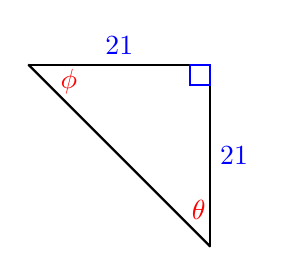
\begin{tikzpicture} 

\coordinate(A) at (0,0);
\coordinate (B) at (0,-2.3 );
\coordinate (C) at (-2.3,0);

\draw[black,thick] (A)--(B) node[right,midway] {\color{blue}$21$};
\draw[black,thick] (A)--(C) node[above,midway] {\color{blue}$21$};
\draw[black,thick] (C)--(B);

\draw[blue,thick] (A) rectangle +(-.25,-.25);
\filldraw[black] (B) circle (.2pt) node[anchor= south east,xshift=2,yshift=6] {\color{red}$\theta$};
\filldraw[black] (C) circle (.2pt) node[anchor= north west,xshift=8,yshift=2] {\color{red}$\phi$};

\end{tikzpicture}
\newline


Chap 1 review 7
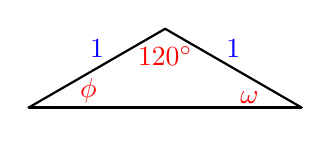
\begin{tikzpicture} 

\coordinate(A) at (0,0);
\coordinate (B) at (1.732,-1);
\coordinate (C) at (-1.732,-1);

\draw[black,thick] (A)--(B) node[above,midway] {\color{blue}$1$};
\draw[black,thick] (A)--(C) node[above,midway] {\color{blue}$1$};
\draw[black,thick] (C)--(B);

\filldraw[black] (A) circle (.2pt) node[anchor= north,xshift=0,yshift=-3] {\color{red}$120\degree$};
\filldraw[black] (B) circle (.2pt) node[anchor= south east,xshift=-12,yshift=-2] {\color{red}$\omega$};
\filldraw[black] (C) circle (.2pt) node[anchor= south west,xshift=15,yshift=-2] {\color{red}$\phi$};

\end{tikzpicture}
\newline


Chap 1 review 8
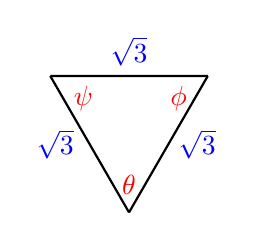
\begin{tikzpicture} [rotate=60]

\coordinate (O) at (0,0);
\coordinate (A) at (2,0);
\coordinate (B) at (1,1.732);

\draw[black,  thick] (O) --  (A) node[right, midway, xshift=0] {\color{blue}$\sqrt{3}$}  ;
\draw[black,  thick] (O) --  (B) node[ left,midway, xshift=-2] {\color{blue}$\sqrt{3}$}  ;
\draw[black,  thick] (A) --  (B) node[above ,midway] {\color{blue}$\sqrt{3}$}  ;
\node at (O) [anchor=south, yshift=3] {\color{red}$\theta$};
\node at (A) [anchor=north east, xshift=-4] {\color{red}$\phi$};
\node at (B) [anchor=north west, xshift=5] {\color{red}$\psi$};

\end{tikzpicture}
\newline


Chap 1 review 9
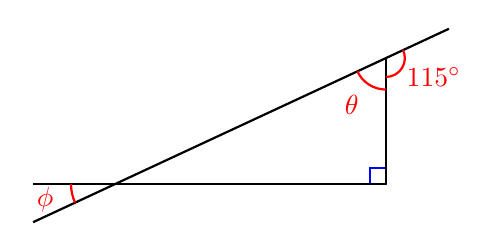
\begin{tikzpicture} [scale=0.8]

\coordinate (O) at (0,0);
\coordinate (y) at (0,2);
\coordinate (x) at (-4.3,0);

\draw[blue,  thick] (O) rectangle  +(-.25,.25)  ;
\draw[black,  thick] (-5.6,0) --  (O)  ;
\draw[black,  thick] (O) --  (y)   ;
\draw[black,  thick] (-5.6,-0.605) --  (1,2.465)  ;
\draw[red, thick] (0,1.7) arc (-90:{atan(2/4.3)}:.3) node [below right, midway,xshift=-2,yshift=4] {$115\degree$};
\draw[red, thick] (0,1.5) arc (-90:{atan(2/4.3)-180}:.5) node [below left, midway,xshift=0,yshift=0] {$\theta$};
\draw[red, thick] (-5,0) arc (180:{atan(2/4.3)+180}:0.7) node [below left, midway,xshift=-3,yshift=6] {$\phi$};

\end{tikzpicture}
\newline


Chap 1 review 10
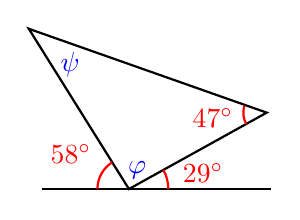
\begin{tikzpicture} 

\coordinate (O) at (0,0);
\coordinate (A) at (1.75,0.97);
\coordinate (B) at (-1.272,2.035);

\filldraw (O) circle (.2pt) node[anchor=south, xshift=3] {\color{blue}$\varphi$};
\filldraw (B) circle (.2pt) node[anchor=north west, xshift=8,yshift=-5] {\color{blue}$\psi$};

\draw[black,  thick] (O) --  (A) --(B)--cycle  ;
\draw[black,  thick] (-1.1,0) --  (1.8,0)  ;
\draw[red, thick] (0.5,0) arc (0:29:.5) node [above right, midway,xshift=2,yshift=-5] {$29\degree$};
\draw[red, thick] (-.4,0) arc (180:122:.4) node [above left, midway,xshift=0,yshift=0] {$58\degree$};
\draw[red, thick] (1.49,0.824) arc (209:{180-atan(.935/3)}:.3) node [ left, midway,xshift=0,yshift=-1] {$47\degree$};

\end{tikzpicture}
\newline


Chap1rev11
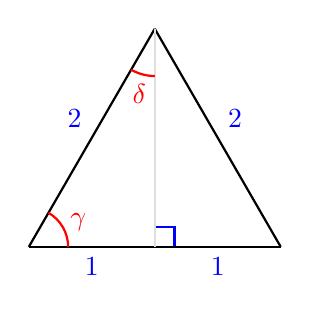
\begin{tikzpicture}

\coordinate (O) at (0,0);
\coordinate (A) at (3.2,0);
\coordinate (B) at (1.6,2.77);
\coordinate (C) at (1.6,0);

\draw[blue,thick] (C) rectangle +(0.25,0.25);
\draw[black,  thick] (O) --  (C) node[below,midway] {\color{blue}$1$}  ;
\draw[black,  thick] (A) --  (C) node[below,midway] {\color{blue}$1$}  ;
\draw[black,  thick] (O) --  (B) node[above left,midway] {\color{blue}$2$}  ;
\draw[black,  thick] (A) --  (B) node[above right,midway] {\color{blue}$2$}  ;
\draw[gray!50!white!50,  thick] (C) --  (B)  ;
\draw[red, thick] (0.5,0) arc (0:60:.5) node [above right, midway,xshift=-1,yshift=-5] {$\gamma$};
\draw[red, thick] (1.6,2.17) arc (-90:-120:.6) node [below left, midway,xshift=5,yshift=0] {$\delta$};

\end{tikzpicture}
\newline


Chap1rev12
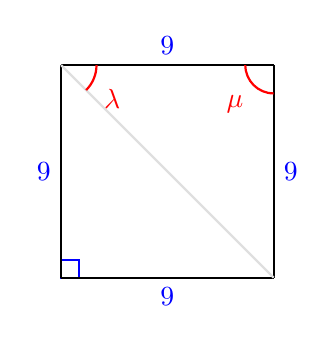
\begin{tikzpicture} [scale=.9]

\coordinate (O) at (0,0);
\coordinate (A) at (3,0);
\coordinate (B) at (3,3);
\coordinate (C) at (0,3);

\draw[blue,thick] (O) rectangle +(0.25,0.25);
\draw[black,  thick] (O) --  (A) node[below,midway] {\color{blue}$9$}  ;
\draw[black,  thick] (A) --  (B) node[right,midway] {\color{blue}$9$}  ;
\draw[black,  thick] (C) --  (B) node[ above,midway] {\color{blue}$9$}  ;
\draw[black,  thick] (C) --  (O) node[left,midway] {\color{blue}$9$}  ;
\draw[gray!50!white!50,  thick] (C) --  (A)  ;
\draw[red, thick] (2.6,3) arc (180:270:.4) node [below left, midway,xshift=0,yshift=0] {$\mu$};
\draw[red, thick] (0.5,3) arc (0:-45:.5) node [below right, midway,xshift=0,yshift=0] {$\lambda$};

\end{tikzpicture}
\newline


Chap1rev13
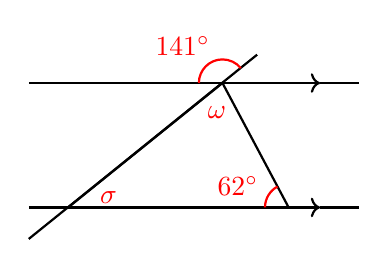
\begin{tikzpicture} 

\coordinate (O) at (0,0);
\coordinate (A) at (2.8,0);
\coordinate (B) at (1.96,1.58);

\draw[black,  thick,->] (-.5,0) --  (3.2,0)  ;
\draw[black,  thick,->] (-.5,1.58) --  (3.2,1.58)  ;
\draw[black,  thick] (3.2,0) -- +(.5,0) ;
\draw[black,  thick] (3.2,1.58) -- +(.5,0)  ;
\draw[black,  thick] (-.5,-.4) --  (2.4,1.94)  ;
\draw[black,  thick] (A) --  (B)  ;
\draw[black,  thick] (O) --  (B)  ;
\draw[red, thick] (2.5,0) arc (180:118:.3) node [above left, midway,xshift=0,yshift=-4] {$62\degree$};
\draw[red, thick] (1.66,1.58) arc (180:39:.3) node [above left, midway, xshift=2,yshift=-2] {$141\degree$};
\filldraw[black] (O) circle (.2pt) node[anchor=south west,xshift=8,yshift=-2] {\color{red}$\sigma$};
\filldraw[black] (B) circle (.2pt) node[anchor=north,xshift=-2,yshift=-5] {\color{red}$\omega$};

\end{tikzpicture}
\newline



Chap1rev14
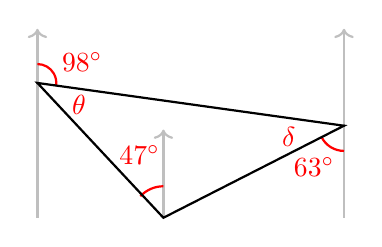
\begin{tikzpicture} [scale=.8]

\coordinate (O) at (0,0);
\coordinate (A) at (-2,2.14);
\coordinate (B) at (2.867,1.461);

\draw[gray!50!white,  thick,->] (-2,0) --  (-2,3)  ;
\draw[gray!50!white,  thick,->] (O) --  +(0,1.4)  ;
\draw[gray!50!white,  thick,->] (2.867,0) --  (2.867,3)  ;
\draw[red, thick] (-2,2.44) arc (90:-8:.3) node [above right, midway,xshift=0,yshift=-4] {$98\degree$};
\draw[red, thick] (2.867,1.061) arc (-90:-153:.4) node [below left, midway, xshift=5,yshift=0] {$63\degree$};
\draw[red, thick] (0,.5) arc (90:137:.5) node [above left, midway, xshift=7,yshift=5] {$47\degree$};
\filldraw[black] (A) circle (.2pt) node[anchor=north west,xshift=9,yshift=-1] {\color{red}$\theta$};
\filldraw[black] (B) circle (.2pt) node[anchor=east,xshift=-14,yshift=-4] {\color{red}$\delta$};
\draw[black,thick] (O)--(A)--(B)--cycle;

\end{tikzpicture}
\newline


Chap1rev15
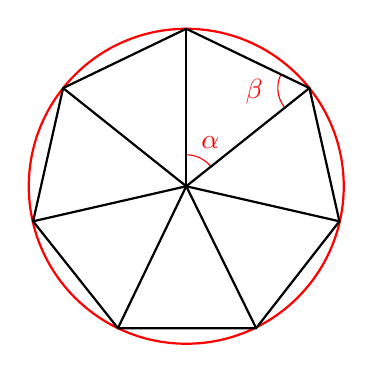
\begin{tikzpicture}
\coordinate(O) at (0,0);
\coordinate (A) at (0,2 );
\coordinate (B) at (1.564,1.247);
\coordinate (C) at(1.945,-0.445);
\coordinate (D) at (0.8878,-1.802);
\coordinate (E) at(-0.8678,-1.802);
\coordinate (F) at(-1.945,-0.445);
\coordinate (G) at(-1.564,1.247);

\draw[red,thick] (0,0) circle (2);
\draw[red] (0,0.4) arc(90:38.57:0.4) node[above right,midway, xshift=-3, yshift=0]{$\alpha$};
\draw[red] (1.25,0.998) arc(218.57:154.29:0.4) node[left, midway,xshift=-2, yshift=0]{$\beta$};

\draw[black,  thick] (A) -- (B) --( C) --(D) --(E)--(F) -- (G)--cycle;
\draw[black,  thick] (B) --  (O);
\draw[black,  thick] (C) --  (O);
\draw[black,  thick] (A)--(O);
\draw[black,  thick] (D) --  (O);
\draw[black,  thick] (E)--(O);
\draw[black,  thick] (F)--(O);
\draw[black,  thick] (G)--(O);

\end{tikzpicture}
\newline


Chap1rev16
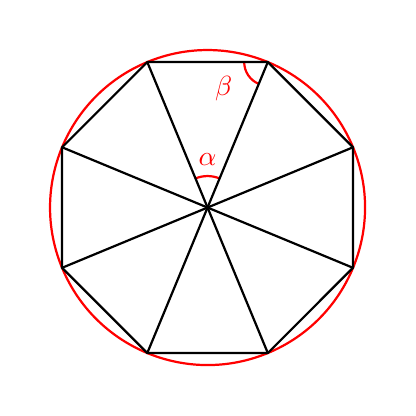
\begin{tikzpicture} [rotate=22.5]
\coordinate(O) at (0,0);
\coordinate (A) at (2,0 );
\coordinate (B) at (1.414,1.414);
\coordinate (C) at(0,2);
\coordinate (D) at (-1.414,1.414);
\coordinate (E) at(-2,0);
\coordinate (F) at(-1.414,-1.414);
\coordinate (G) at(0,-2);
\coordinate (H) at (1.414,-1.414);

\draw[red,thick] (0,0) circle (2);
\draw[red,thick] (0,0.4) arc(90:45:0.4) node[above,midway, xshift=0, yshift=0]{$\alpha$};
\draw[red,thick] (1.202,1.202) arc(225:157.5:0.3) node[left, midway,xshift=-2, yshift=-5]{$\beta$};

\draw[black,  thick] (A) -- (B) --( C) --(D) --(E)--(F) -- (G)--(H)--cycle;
\draw[black,  thick] (B) --  (O);
\draw[black,  thick] (C) --  (O);
\draw[black,  thick] (A)--(O);
\draw[black,  thick] (D) --  (O);
\draw[black,  thick] (E)--(O);
\draw[black,  thick] (F)--(O);
\draw[black,  thick] (G)--(O);
\draw[black,  thick] (H)--(O);

\end{tikzpicture}
\newline


Chap1rev17
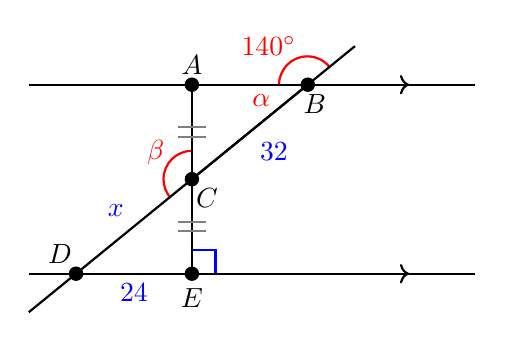
\begin{tikzpicture} [scale=1.2]
\coordinate (A) at (0,1 );
\coordinate (B) at (1.226,1);
\coordinate (C) at (0,0);
\coordinate (D) at (-1.226,-1);
\coordinate (E) at (0,-1);

\filldraw[black] (A) circle (2pt) node[anchor=south] {$A$};
\filldraw[black] (B) circle (.2pt) node[anchor=north west, xshift=-5] {$B$};
\filldraw[black] (B) circle (2pt) node[anchor=north east, xshift=-10, yshift=0] {\color{red}$\alpha$};
\filldraw[black] (C) circle (2pt) node[anchor=north west, xshift=-2] {$C$};

\filldraw[black] (D) circle (2pt) node[anchor=south east, xshift=2] {$D$};
\filldraw[black] (E) circle (2pt) node[anchor=north, yshift=-2] {$E$};

\draw[red,thick] (0.9226,1) arc(180:{atan(1/1.226)}:0.3) node[above left,midway, xshift=3, yshift=-3]{$140\degree$};
\draw[red,thick] (0,0.3) arc(90:{atan(1/1.226)+180}:0.3) node[above left,midway, xshift=3, yshift=-3]{$\beta$};

\draw[blue, thick] (E) rectangle +(0.25,0.25);
\draw[black,  thick] (-1.726,1)--(3,1);
\draw[black,  thick] (-1.726,-1)--(3,-1);

\draw[black,  thick] (B) --  (C) node[below right,midway] {\color{blue}$32$};
\draw[black,  thick] (C) --  (D) node[above left,midway] {\color{blue}$x$};
\draw[black,  thick] (A)--(E);
\draw[black,  thick] (D) --  (E) node[below,midway] {\color{blue}$24$};
\draw[black,  thick] (B)--(C);
\draw[black, thick] (D) -- +(-.5,-.4078);
\draw[black, thick] (B) -- +(.5,.4078);

\draw[gray,thick] (-.15, .45) -- +(.3,0);
\draw[gray,thick] (-.15, .55) -- +(.3,0);
\draw[gray,thick] (-.15, -.45) -- +(.3,0);
\draw[gray,thick] (-.15, -.55) -- +(.3,0);

\draw[black, thick, ->] (A)-- +(2.3,0);
\draw[black, thick, ->] (E)-- +(2.3,0);

\end{tikzpicture}
\newline


Chap1rev18
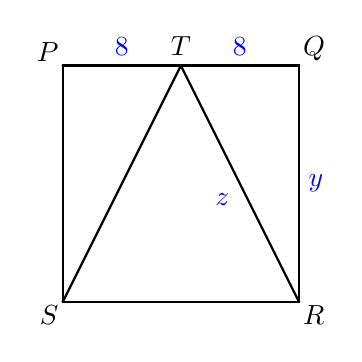
\begin{tikzpicture} 
\coordinate(S) at (0,0);
\coordinate (R) at (3,0 );
\coordinate (Q) at (3,3);
\coordinate (P) at(0,3);
\coordinate (T) at (1.5,3);

\filldraw[black] (P) circle (.2pt) node[anchor=south east, xshift=2, yshift=-2] {$P$};
\filldraw[black] (Q) circle (.2pt) node[anchor=south west, xshift=-2, yshift=-2] {$Q$};
\filldraw[black] (R) circle (.2pt) node[anchor=north west, xshift=-2, yshift=2] {$R$};
\filldraw[black] (S) circle (.2pt) node[anchor=north east, xshift=2, yshift=2] {$S$};
\filldraw[black] (T) circle (.2pt) node[anchor=south, xshift=0, yshift=0] {$T$};

\draw[black,  thick] (P) -- (Q) --( R) --(S)--cycle;
\draw[black,  thick] (S) --  (T);
\draw[black,  thick] (R) --  (T) node[below left,midway] {\color{blue}$z$};

\node at (0.75,3) [anchor=south] {\color{blue}$8$};
\node at (2.25,3) [anchor=south] {\color{blue}$8$};
\node at (3,1.5) [anchor=west] {\color{blue}$y$};

\end{tikzpicture}
\newline


Chap1rev19
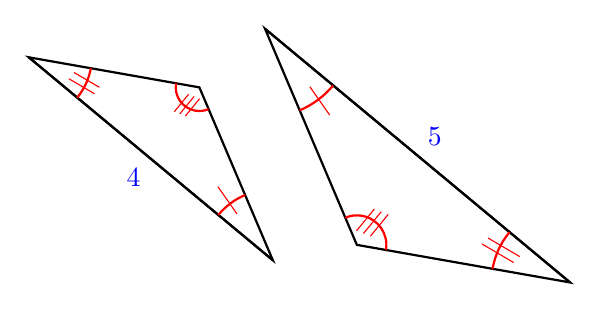
\begin{tikzpicture}

\draw[black, thick, rotate=170] (0,0) --  (2.2,0) --(-1.3,2)--cycle ;
\draw[black, thick, rotate=170] (2.2,0) --(-1.3,2) node [below left,midway] {\color{blue}$4$} ;
\draw[red, thick, rotate=170] (0.3,0) arc(0:{180-atan(2/1.3)}:0.3);
\draw[red, rotate=170] (.12,.11) -- +(.14,.25);
\draw[red, rotate=170] (.046,.125) -- +(.14,.25);
\draw[red, rotate=170] (-.028,.14) -- +(.14,.25);

\draw[red, thick, rotate=170] (1.4,0) arc(180:{180-atan(2/3.5)}:0.8);
\draw[red, rotate=170] (1.6,.09) -- +(-.35,.13);
\draw[red, rotate=170] (1.65,.18) -- +(-.35,.13);

\draw[red, thick, rotate=170] (-.8095,1.245) arc({atan(-2/1.3)}:{-atan(2/3.5)}:0.9);
\draw[red, rotate=170] (-.75,1.5) -- +(.3,-.3);

\draw[black,  thick, shift={(2 cm, -2 cm)},scale=1.25, rotate=-10]   (0,0) --  (2.2,0) --(-1.3,2)--cycle ;
\draw[black, thick,  shift={(2 cm, -2 cm)},scale=1.25, rotate=-10] (2.2,0) --(-1.3,2) node [above right,midway] {\color{blue}$5$} ;
\draw[red, thick, shift={(2 cm, -2 cm)},scale=1.25, rotate=-10] (0.3,0) arc(0:{180-atan(2/1.3)}:0.3);
\draw[red, shift={(2 cm, -2 cm)},scale=1.25, rotate=-10] (.12,.11) -- +(.14,.25);
\draw[red, shift={(2 cm, -2 cm)},scale=1.25, rotate=-10]  (.046,.125) -- +(.14,.25);
\draw[red, shift={(2 cm, -2 cm)},scale=1.25, rotate=-10]  (-.028,.14) -- +(.14,.25);

\draw[red, thick, shift={(2 cm, -2 cm)},scale=1.25, rotate=-10] (1.4,0) arc(180:{180-atan(2/3.5)}:0.8);
\draw[red,shift={(2 cm, -2 cm)},scale=1.25, rotate=-10] (1.6,.10) -- +(-.35,.13);
\draw[red, shift={(2 cm, -2 cm)},scale=1.25, rotate=-10] (1.65,.17) -- +(-.35,.13);

\draw[red, thick, shift={(2 cm, -2 cm)},scale=1.25, rotate=-10] (-.8095,1.245) arc({atan(-2/1.3)}:{-atan(2/3.5)}:0.9);
\draw[red, shift={(2 cm, -2 cm)},scale=1.25, rotate=-10] (-.75,1.5) -- +(.25,-.25);

\end{tikzpicture}
\newline


Chap1rev20
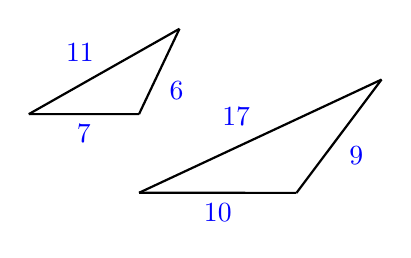
\begin{tikzpicture} 

\draw[black, thick, scale=.2,rotate=64.62] (0,0) -- (6,0) node[below right,midway] {\color{blue}$6$};
\draw[black, thick, scale=.2,rotate=64.62] (6,0) --( -3,6.3245) node[above left, midway] {\color{blue}$11$};
\draw[black, thick, scale=.2,rotate=64.62] (0,0)  --( -3,6.3245) node[below, midway] {\color{blue}$7$};

\draw[black, thick,xshift=2cm,yshift=-1cm, scale=.2,rotate=53.1] (0,0) -- (9,0) node[below right,midway] {\color{blue}$9$};
\draw[black, thick,xshift=2cm,yshift=-1cm, scale=.2,rotate=53.1] (9,0) --( -6,8) node[above left, midway] {\color{blue}$17$};
\draw[black, thick, xshift=2cm,yshift=-1cm, scale=.2,rotate=53.1] (0,0)  --( -6,8) node[below, midway] {\color{blue}$10$};

\end{tikzpicture}
\newline


Chap1rev21
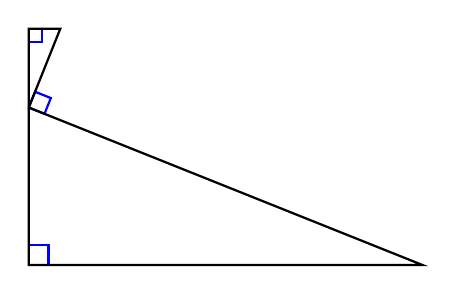
\begin{tikzpicture} 
\coordinate(O) at (0,0);
\coordinate (A) at (5,0 );
\coordinate (B) at (0,2);
\coordinate (C) at (0,3);
\coordinate (D) at (.4,3);

\draw[blue,thick] (O) rectangle +(0.25,0.25);
\draw[blue,thick] (B) -- ++(0.2,-0.08)-- ++(0.08,0.2)-- ++(-0.2,0.08)-- ++(-0.08,-0.2);
\draw[blue,thick] (C) rectangle +(0.17,-0.17);
\draw[black, thick] (O)--(A)--(B)--(D)--(C)--cycle;

\end{tikzpicture}
\newline


Chap1rev22
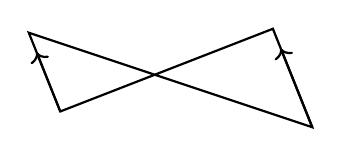
\begin{tikzpicture} 
\coordinate(O) at (0,0);
\coordinate (A) at (3.2,-.2 );
\coordinate (B) at (-0.4,1.0);
\coordinate (C) at (2.7,1.05);

\draw[black,thick] (O) -- (C) --(A)--(B)--cycle;
\draw[black, thick, ->] (O) -- (-.3,.75);
\draw[black, thick, ->] (A) -- (2.8,0.8);

\end{tikzpicture}
\newline


Chap1rev23
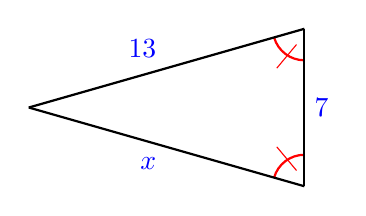
\begin{tikzpicture} 
\coordinate(O) at (0,0);
\coordinate (A) at (3.5,1 );
\coordinate (B) at (3.5,-1);

\draw[red,thick] (3.5,0.6) arc(270:{180+atan(1/3.5}:0.4);
\draw[red] (3.4,.8) -- +(-.25,-.3);
\draw[red,thick] (3.5,-0.6) arc(90:{180-atan(1/3.5}:0.4);
\draw[red] (3.4,-.8) -- +(-.25,.3);

\draw[black,thick] (O) -- (A) node[above left, midway] {\color{blue}$13$};
\draw[black,thick] (A)--(B) node[right,midway] {\color{blue}$7$};
\draw[black,thick] (O) --(B) node [below left, midway] {\color{blue}$x$};

\end{tikzpicture}
\newline


Chap1rev24
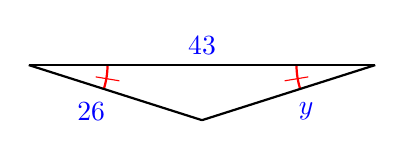
\begin{tikzpicture} 
\coordinate(O) at (0,0);
\coordinate (A) at (2.2,.7 );
\coordinate (B) at (-2.2,.7);

\draw[red,thick] (-1.2,.7) arc(0:{-atan(7/22}:1);
\draw[red] (-1.35,.55) -- +(.3,-.05);
\draw[red,thick] (1.2,.7) arc(180:{180+atan(7/22}:1);
\draw[red] (1.35,.55) -- +(-.3,-.05);

\draw[black,thick] (O) -- (A) node[below right, midway] {\color{blue}$y$};
\draw[black,thick] (A)--(B) node[above,midway] {\color{blue}$43$};
\draw[black,thick] (O) --(B) node [below left, midway] {\color{blue}$26$};

\end{tikzpicture}
\newline


Chap1rev25
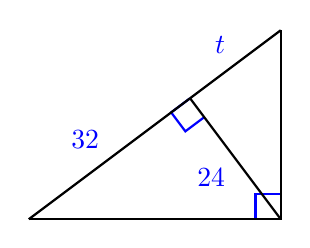
\begin{tikzpicture} [scale=.08]
\coordinate(O) at (0,0);
\coordinate (A) at (40,0 );
\coordinate (B) at (40,30);
\coordinate (C) at (25.6,19.2);

\draw[blue,thick] (A) rectangle +(-4,4);
\draw[blue,thick] (C) -- ++(-3,-2.25)--++(2.25,-3)--++(3,2.25);

\draw[black,thick] (C) -- (A) node[below left, midway] {\color{blue}$24$};
\draw[black,thick] (C)--(B) node[above left,midway] {\color{blue}$t$};
\draw[black,thick] (O) --(C) node [above left, midway] {\color{blue}$32$};
\draw[black,thick] (O)--(A)--(B);

\end{tikzpicture}
\newline


Chap1rev26
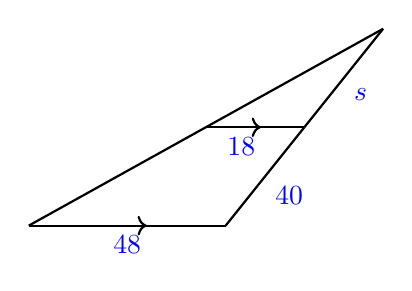
\begin{tikzpicture} 
\coordinate(O) at (0,0);
\coordinate (A) at (2.5,0 );
\coordinate (B) at (4.5,2.5);
\coordinate (C) at (2.25,1.25);
\coordinate (D) at (3.5,1.25);

\draw[black,thick] (O) -- (A) node[below , midway] {\color{blue}$48$};
\draw[black,thick] (A)--(D) node[below right,midway] {\color{blue}$40$};
\draw[black,thick] (D) --(B) node [below right, midway] {\color{blue}$s$};
\draw[black,thick] (D) --(C) node [below, midway, xshift=-5] {\color{blue}$18$};
\draw[black,thick] (O) --(B);
\draw[black,thick,->] (O) -- (1.5,0);
\draw[black,thick,->] (C) -- +(0.7,0);

\end{tikzpicture}
\newline


Chap1rev27
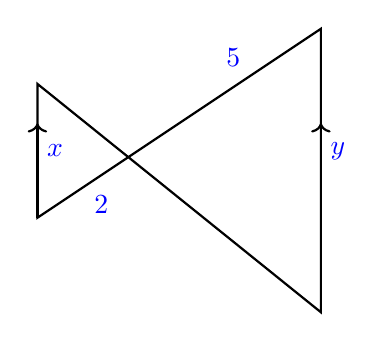
\begin{tikzpicture} 
\coordinate (O) at (0,0);
\coordinate (A) at (0,1.7 );
\coordinate (B) at (3.6,-1.2);
\coordinate (C) at (3.6,2.4);

\draw[black,thick] (O) --(A)--(B)--(C)--cycle;
\draw[black,thick,->] (O) -- +(0,1.2);
\draw[black,thick,->] (B) -- (3.6,1.2);
\node at (0,.85) [anchor=west]{\color{blue}$x$};
\node at (3.6,.85) [anchor=west]{\color{blue}$y$};
\node at (.6,.4) [anchor=north west]{\color{blue}$2$};
\node at (2.7,1.8) [anchor=south east]{\color{blue}$5$};

\end{tikzpicture}
\newline


Chap1rev28
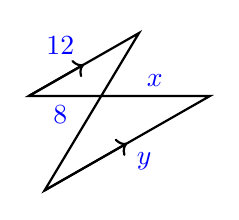
\begin{tikzpicture} 
\coordinate (O) at (0,0);
\coordinate (A) at (2.1,1.2 );
\coordinate (B) at (-.2,1.2);
\coordinate (C) at (1.2,2);

\draw[black,thick] (O) --(A)--(B)--(C)--cycle;
\draw[black,thick,->] (O) -- (1.05,.6);
\draw[black,thick,->] (B) -- +(.7,.4);
\node at (1.4,1.2) [anchor=south]{\color{blue}$x$};
\node at (1.05,.6) [anchor=north west]{\color{blue}$y$};
\node at (.2,1.2) [anchor=north ]{\color{blue}$8$};
\node at (.5,1.6) [anchor=south east]{\color{blue}$12$};

\end{tikzpicture}
\newline


Chap1rev29
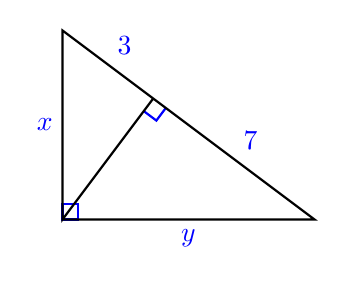
\begin{tikzpicture} [scale=.8]
\coordinate (O) at (0,0);
\coordinate (A) at (4,0 );
\coordinate (B) at (0,3);
\coordinate (C) at (1.44,1.92);

\draw[blue,thick] (O) rectangle +(0.25,0.25);
\draw[blue,thick] (C) ++(-.15,-0.20) -- ++(.20,-.15)--++(.15,.20);

\draw[black,thick] (O) --(A)--(B)--(O)--(C);
\node at (0,1.5) [anchor=east]{\color{blue}$x$};
\node at (2,0) [anchor=north ]{\color{blue}$y$};
\node at (0.72,2.46) [anchor=south west ]{\color{blue}$3$};
\node at (2.72,0.96) [anchor=south west]{\color{blue}$7$};

\end{tikzpicture}
\newline


Chap1rev30
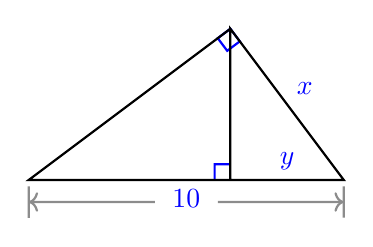
\begin{tikzpicture} [scale=.8,rotate=-{180+atan(3/4)}]
\coordinate (O) at (0,0);
\coordinate (A) at (4,0 );
\coordinate (B) at (0,3);
\coordinate (C) at (1.44,1.92);

\draw[blue,thick] (O) rectangle +(0.25,0.25);
\draw[blue,thick] (C) ++(-.15,-0.20) -- ++(.20,-.15)--++(.15,.20);

\draw[black,thick] (O) --(A)--(B)--(O)--(C);
\node at (0,1.5) [anchor=south west]{\color{blue}$x$};
\node at (0.72,2.46) [anchor=south ]{\color{blue}$y$};
\node at (2,1.5) [anchor=north ]{\color{blue}$10$};
\draw[gray!90!white,thick] (.06,3.08) -- +(.3,.4);
\draw[gray!90!white,thick] (4.06,.08) -- +(.3,.4);
\draw[gray!90!white,thick,<-] (.21,3.28) -- +(1.6,-1.2);
\draw[gray!90!white,thick,<-] (4.21,.28) -- +(-1.6,1.2);

\end{tikzpicture}
\newline


Chap1rev31
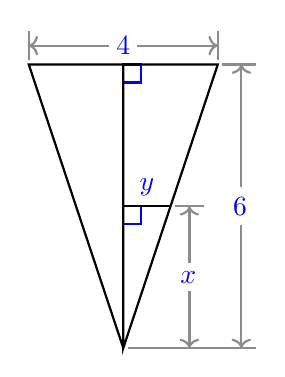
\begin{tikzpicture} [scale=0.6]
\coordinate (O) at (0,0);
\coordinate (A) at (-2,6 );
\coordinate (B) at (2,6);
\coordinate (C) at (0,6);
\coordinate (D) at (0,3);
\coordinate (E) at (1,3);

\draw[blue,thick] (0,6) rectangle +(0.38,-0.38);
\draw[blue,thick] (D) rectangle +(0.38,-0.38);

\draw[black,thick] (O) --(A)--(C)--(O)--(B)--(A);
\draw[black,thick] (D)--(E) node[above,midway] {\color{blue}$y$};
\node at (2,3) [anchor= west,xshift=2]{\color{blue}$6$};
\node at (C) [anchor=south ]{\color{blue}$4$};
\draw[gray!90!white,thick, <-] (-2,6.4) -- +(1.7,0);
\draw[gray!90!white,thick, <-] (2,6.4) -- +(-1.7,0);
\draw[gray!90!white,thick] (-2,6.1) -- +(0,.6);
\draw[gray!90!white,thick] (2,6.1) -- +(0,.6);

\draw[gray!90!white,thick] (.1,0) -- +(2.7,0);
\draw[gray!90!white,thick] (2.1,6) -- +(.7,0);
\draw[gray!90!white,thick,<-] (2.5,6) -- +(0,-2.6);
\draw[gray!90!white,thick,<-] (2.5,0) -- +(0,2.6);

\draw[gray!90!white,thick] (1.1,3) -- +(0.6,0);
\draw[gray!90!white,thick,<-] (1.4,3) -- +(0,-1.2);
\draw[gray!90!white,thick,<-] (1.4,0) -- +(0,1.2);
\node at (1,1.5) [anchor= west,xshift=0]{\color{blue}$x$};

\end{tikzpicture}
\newline


Chap1rev32
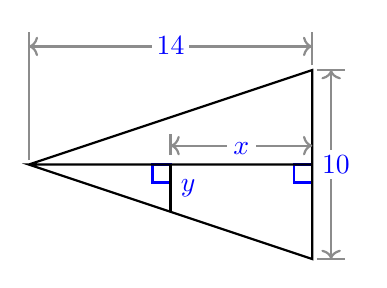
\begin{tikzpicture} [scale=0.6, rotate=-90]
\coordinate (O) at (0,0);
\coordinate (A) at (-2,6 );
\coordinate (B) at (2,6);
\coordinate (C) at (0,6);
\coordinate (D) at (0,3);
\coordinate (E) at (1,3);

\draw[blue,thick] (0,6) rectangle +(0.38,-0.38);
\draw[blue,thick] (D) rectangle +(0.38,-0.38);

\draw[black,thick] (O) --(A)--(C)--(O)--(B)--(A);
\draw[black,thick] (D)--(E) node[right, midway] {\color{blue}$y$};
\node at (-2,3) [anchor= south,yshift=2]{\color{blue}$14$};
\node at (C) [anchor=west ]{\color{blue}$10$};
\draw[gray!90!white,thick, <-] (-2,6.4) -- +(1.7,0);
\draw[gray!90!white,thick, <-] (2,6.4) -- +(-1.7,0);
\draw[gray!90!white,thick] (-2,6.1) -- +(0,.6);
\draw[gray!90!white,thick] (2,6.1) -- +(0,.6);

\draw[gray!90!white,thick] (-.1,0) -- +(-2.7,0);
\draw[gray!90!white,thick] (-2.1,6) -- +(-.7,0);
\draw[gray!90!white,thick,<-] (-2.5,6) -- +(0,-2.6);
\draw[gray!90!white,thick,<-] (-2.5,0) -- +(0,2.6);

\node at (0,4.5) [anchor= south,yshift=0]{\color{blue}$x$};
\draw[gray!90!white,thick,<-] (-0.4,6) -- +(0,-1.2);
\draw[gray!90!white,thick,<-] (-0.4,3) -- +(0,1.2);
\draw[gray!90!white,thick] (-0.2,3) -- +(-0.45,0);

\end{tikzpicture}
\newline



Chap1rev33
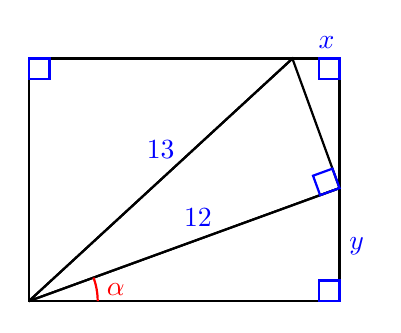
\begin{tikzpicture} [scale=.35]
\coordinate (O) at (0,0);

\draw[black,thick,rotate=20] (O) --(12,0)--(12,5)--(O);
\draw[black,thick,rotate=20] (O) --(12,0) node[above,midway, xshift=5pt,yshift=3] {\color{blue}$12$};
\draw[black,thick,rotate=20] (O) --(12,5) node[above,midway, xshift=0pt,yshift=4] {\color{blue}$13$};

\coordinate (A) at (11.2763,0 );
\coordinate (B) at (11.2763,8.8027);
\coordinate(C) (11.2763, 4.1042);
\coordinate(D) (9.5662, 8.8027);
\coordinate (E) at (0,8.8027);

\draw[black,thick] (O) rectangle (B);
\draw[blue,thick] (A) rectangle +(-.75,.75);
\draw[blue,thick] (B) rectangle +(-.75,-.75);
\draw[blue,thick] (E) rectangle +(.75,-.75);
\draw[blue,thick,rotate=20] (12,0) rectangle +(-.75,.75);

\node [anchor=west] at (11.2763,2) {\color{blue}$y$};
\node [anchor=south] at (10.8,8.8027) {\color{blue}$x$};

\draw[red,thick] (2.5,0) arc (0:20: 2.5) node[right, midway] {$\alpha$};

\end{tikzpicture}
\newline


Chap1rev34
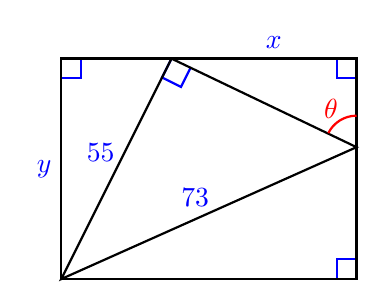
\begin{tikzpicture}
\coordinate (O) at (0,0);
\coordinate (A) at (3.75,0 );
\coordinate (B) at (3.75,2.8);
\coordinate (C) at (0,2.8);
\coordinate (D) at (1.4, 2.8);
\coordinate (E) at (3.75,1.675);

\draw[blue,thick] (A) rectangle +(-0.25,0.25);
\draw[blue,thick] (B) rectangle +(-0.25,-0.25);
\draw[blue,thick] (C) rectangle +(0.25,-0.25);
\draw[blue,thick] (D) -- ++(-0.12,-0.24) -- ++(0.24,-0.12)-- ++(0.12,0.24);

\draw[black,thick] (O) rectangle (B);
\draw[black,thick] (O) -- (D) -- (E) -- cycle;

\node [anchor=south east] at (2,0.8)  {$\color{blue}73$};
\node [anchor=east] at (0.8,1.6)  {$\color{blue}55$};
\node [anchor=east] at (0,1.4) {\color{blue}$y$};
\node [anchor=south] at (2.7,2.8) {\color{blue}$x$};
\draw[red,thick] (3.75,2.075) arc (90:{180-atan(.5)}: 0.4) node[above left, midway,xshift=3,yshift=-3] {$\theta$};

\end{tikzpicture}
\newline


Chap1rev35
\usetikzlibrary{arrows.meta}
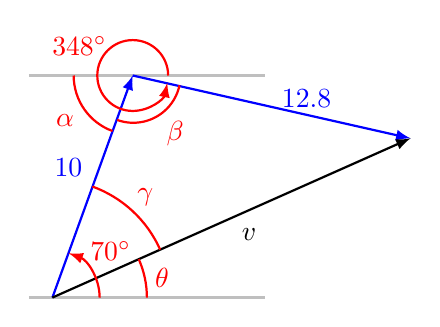
\begin{tikzpicture} [scale=.3]
\coordinate (O) at (0,0);
\coordinate (A) at (3.4,9.4 );
\coordinate (B) at (15.16,6.74);

\draw[gray!50!white,thick] (-1,0) -- +(10,0);
\draw[gray!50!white,thick] (-1,9.4) -- +(10,0);

\draw[blue,thick,>=latex,->] (O) -- (A) node [above left, midway] {$10$};
\draw[blue,thick,>=latex,->] (A) -- (B) node [above right, midway, yshift=-4] {$12.8$};
\draw[black,thick,>=latex,-{>  [length=20,width=20]}] (O) -- (B) node[below right,midway] {$v$};

\draw[red,thick,->,>=latex] (2,0) arc (0:70:2) node [above right, midway, xshift=-4] {$70\degree$};
\draw[red,thick] (4,0) arc (0:{atan(6.74/15.16)}:4) node [right, midway, xshift=0] {$\theta$};
\draw[red,thick] (4.56,2.03) arc ({atan(6.74/15.16)}:{atan(94/34)}:5) node [above right, midway, xshift=-2,yshift=-2] {$\gamma$};
\draw[red,thick,->,>=latex] (4.9,9.4) arc (0:348:1.5) node [above left, midway, xshift=7,yshift=2] {$348\degree$};
\draw[red,thick] (2.74,7.52) arc ({250}:348:2) node [below right, midway, xshift=0,yshift=2] {$\beta$};
\draw[red,thick] (0.9,9.4) arc (180:250:2.5) node [below left, midway, xshift=0,yshift=2] {$\alpha$};

\end{tikzpicture}
\newline


Chap1rev36
\usetikzlibrary{arrows.meta}
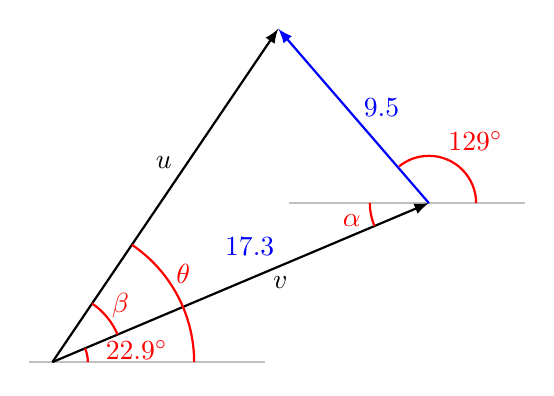
\begin{tikzpicture} [scale=.3]
\coordinate (O) at (0,0);
\coordinate (A) at (15.937,6.732 );
\coordinate (B) at (9.56,14.11);

\draw[gray!50!white,thick] (-1,0) -- +(10,0);
\draw[gray!50!white,thick] (10,6.732) -- +(10,0);

\draw[black,thick,>=latex,->] (O) -- (A) node [below right, midway, xshift=8,yshift=6] {$v$};
\draw[blue,thick,>=latex,->] (A) -- (B) node [above right, midway, yshift=-4] {$9.5$};
\draw[black,thick,>=latex,-{>  [length=20,width=20]}] (O) -- (B) node[above left,midway,xshift=6,yshift=6] {$u$};

\node [anchor=south, xshift=3,yshift=6] at (8,3.4) {\color{blue}$17.3$};

\draw[red,thick] (17.937,6.732) arc (0:129:2) node [above right, midway, xshift=-4] {$129\degree$};
\draw[red,thick] (6,0) arc (0:{atan(14.11/9.56)}:6) node [midway, xshift=2, yshift=8] {$\theta$};
\draw[red,thick] (1.5,0) arc (0:22.9:1.5) node [right, midway, xshift=3,yshift=2] {$22.9\degree$};
\draw[red,thick] (1.68,2.48) arc ({atan(14.11/9.56)}:22.9:3) node [above right, midway, xshift=-2,yshift=-4] {$\beta$};
\draw[red,thick] (13.437,6.732) arc (180:202.9:2.5) node [left, midway, xshift=0,yshift=-2] {$\alpha$};

\end{tikzpicture}
\newline


\section {Stuff for later}
Section 4.2 Angle of inclination
\begin{tikzpicture}

\coordinate (O) at (0,0);
\coordinate (x) at (3.5,0);
\coordinate (y) at (0,2);
\coordinate (A) at (3,1.8);
\coordinate (B) at (1.,0);
\coordinate (C) at (2.5,0);
\coordinate (D) at (-1,-1.8);

\draw[black,  thick, ->] (-1.5,0) --  (x) node[right] {$x$} ;
\draw[black,  thick, ->] (0,-2) --  (y) node[above] {$y$}  ;
\draw[black,  thick, <->] (D) --  (A)  ;
\draw[red, thick] (1.9,0) arc (0:{atan(0.9)}:.9) node [left, midway,xshift=0,yshift=-3] {$\alpha$};

\end{tikzpicture}
\newline

Section 4.2 Angle of inclination
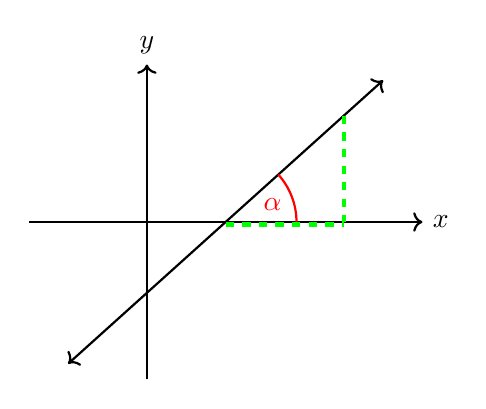
\begin{tikzpicture}

\coordinate (O) at (0,0);
\coordinate (x) at (3.5,0);
\coordinate (y) at (0,2);
\coordinate (A) at (3,1.8);
\coordinate (B) at (1.,0);
\coordinate (C) at (2.5,0);
\coordinate (D) at (-1,-1.8);

\draw[black,  thick, ->] (-1.5,0) --  (x) node[right] {$x$} ;
\draw[black,  thick, ->] (0,-2) --  (y) node[above] {$y$}  ;
\draw[black,  thick, <->] (D) --  (A)  ;
\draw[red, thick] (1.9,0) arc (0:{atan(0.9)}:.9) node [left, midway,xshift=0,yshift=-3] {$\alpha$};

\draw[green, ultra thick, dashed] (1,-.03) -- (2.5,-.03);
\draw[green, ultra thick, dashed] (2.5,1.35) -- (2.5,0);

\end{tikzpicture}
\newline


Exercise not used?
\begin{tikzpicture}
\coordinate (O) at (0,0);
\coordinate (A) at (0,0);
\coordinate (B) at (0,0);
\coordinate(C) at (0,0);
\coordinate (D) at (0,0);
\filldraw[black] (O) circle (.2pt) node[anchor=south west, xshift=6]{$50\degree$};
\filldraw[black] (A) circle (.2pt) node[anchor=south east]{$x$};
\filldraw[black] (B) circle (.2pt) node[anchor=north east, xshift=-6]{$y$};
\filldraw[black] (C) circle (.2pt) node[anchor=north west]{$z$};
%\draw[black,  thick] (A) -- (B) --( C) -- cycle;
\draw[black] (-2.3,0) --  (2.3,0);
\draw[black] (0.8,1.3) --  (-0.8,-1.3) ;
\end{tikzpicture}
\newline


\end{document}
